\documentclass[11pt,a4paper]{article}

\usepackage[margin=22mm,headheight=15pt]{geometry}
\usepackage[T1]{fontenc}
\usepackage{lmodern}
\usepackage{microtype}
\usepackage{amsmath,amssymb}
\usepackage{siunitx}
\usepackage{booktabs}
\usepackage{graphicx}
\usepackage{float}
\usepackage{enumitem}
\usepackage{xcolor}
\usepackage{caption}
\usepackage{fancyhdr}
\usepackage[hidelinks]{hyperref}

\definecolor{navy}{HTML}{17365D}
\definecolor{rulegray}{HTML}{B8C2CC}
\hypersetup{
  pdftitle={Saturation Temperature and Pressure Report 2026},
  pdfauthor={Aaron Taylor},
  pdfsubject={ENME 601 Thermodynamics Laboratory 1},
  pdfkeywords={saturation pressure, PT100, steam tables, thermodynamics}
}
\captionsetup{font=small,labelfont=bf,justification=centering}
\sisetup{round-mode=places,round-precision=2,detect-all}
\setlist[itemize]{leftmargin=6mm,itemsep=1.5pt,topsep=3pt}
\setlist[enumerate]{leftmargin=7mm,itemsep=2pt,topsep=3pt}
\setlength{\parindent}{0pt}
\setlength{\parskip}{4pt}
\setlength{\tabcolsep}{4.5pt}
\setlength{\emergencystretch}{1.5em}

\pagestyle{fancy}
\fancyhf{}
\fancyhead[L]{\small ENME 601 Thermodynamics}
\fancyhead[R]{\small Saturation Temperature and Pressure}
\fancyfoot[C]{\thepage}
\renewcommand{\headrulewidth}{0.4pt}
\newcommand{\sectionrule}{\vspace{-2pt}\color{rulegray}\hrule\color{black}\vspace{5pt}}

\begin{document}

\begin{center}
  {\LARGE\bfseries Saturation Temperature and Pressure Lab}\par
  \vspace{3mm}
  {\large Aaron Taylor --- 24232594}\par
  \vspace{1.5mm}
  {\large 1 August 2026}\par
\end{center}
\vspace{4mm}

\section*{Synopsis}
\sectionrule
The relationship between the saturation temperature and absolute pressure of
water was investigated using an Armfield TH3 saturation-pressure apparatus.
Nine equilibrium-stage readings were recorded from \SI{50}{\kilo\pascal} to
\SI{450}{\kilo\pascal} gauge pressure. The measured atmospheric pressure of
\SI{101.65}{\kilo\pascal} was added to each gauge reading. The original PT100
resistance readings were converted using the two-point relationship recorded
on the laboratory whiteboard for this session: $109.0~\Omega$ at
$15\,{}^\circ\mathrm{C}$ and $138.7~\Omega$ at $100\,{}^\circ\mathrm{C}$.

Both the experimental and published steam-table data followed a smooth power
relationship of the form $T=AP^n$. The experimental fit was
$T=37.633P^{0.2146}$, compared with $T=31.019P^{0.2557}$ for the direct
steam-table values. Experimental temperatures were below point-specific
interpolated theoretical values at all nine pressures. The mean signed error
was $-4.32\%$, and the largest absolute error was $6.47\%$. The experiment
reproduced the expected increasing saturation trend, but the growing negative
deviation indicates a systematic influence. Plausible contributors include
thermal lag, heat loss, residual air and uncertainty introduced by the
session-supplied linear conversion. Repeated readings at each pressure would
be required to separate repeatability from systematic bias.

\section{Aim}
\sectionrule
To measure the relationship between the saturation temperature and absolute
pressure of water, determine an empirical power-law model, and assess the
accuracy of the apparatus by comparison with published saturated-water data.

\section{Theory and Data Processing}
\sectionrule
At liquid--vapour equilibrium, saturated liquid water and saturated steam have
one saturation temperature for a given absolute pressure. Increasing pressure
raises this temperature and produces a smooth, nonlinear saturation curve.
The electronic pressure reading was gauge pressure, therefore
\begin{equation}
  P_{\mathrm{abs}}=P_1+P_{\mathrm{atm}},
  \qquad P_{\mathrm{atm}}=\SI{101.65}{\kilo\pascal}.
  \label{eq:pressure}
\end{equation}

The laboratory whiteboard explicitly supplied two resistance--temperature
points for processing this session's readings:
\begin{equation}
 \alpha=\frac{R_2-R_1}{T_2-T_1}
 =\frac{138.7-109.0}{100-15}
 =0.34941~\Omega/{}^\circ\mathrm{C}.
 \label{eq:session-calibration}
\end{equation}
The experimental temperature was therefore calculated as
\begin{equation}
 T_{\mathrm{exp}}=T_1+\frac{R-R_1}{\alpha}
 =15+\frac{R-109.0}{0.34941}.
 \label{eq:pt100}
\end{equation}
This is the method documented in the primary evidence from the actual laboratory
session. It differs from the manufacturer's general Data Sheet~1 bridge
correction followed by the Data Sheet~2 PT100 reference chart. The session
relationship was retained so the report reproduces the experiment as instructed;
the difference from the manual is treated as a methodological limitation rather
than concealed as an apparatus calibration.

Over the measured range, both datasets were represented by
\begin{equation}
  T_{\mathrm{sat}}=AP_{\mathrm{sat}}^n,
  \label{eq:power}
\end{equation}
where $A$ and $n$ were obtained by a log-space least-squares fit. Direct values
from saturated-water pressure Table A--5 were used for the comparison curve.
For the error calculation only, the theoretical temperature at each
experimental pressure was found by linear interpolation:
\begin{equation}
  T_{\mathrm{th}}=T_a+\frac{P_{\mathrm{abs}}-P_a}{P_b-P_a}(T_b-T_a).
  \label{eq:interpolation}
\end{equation}
The signed percentage error was
\begin{equation}
  \mathrm{Error}\ (\%)=\frac{T_{\mathrm{exp}}-T_{\mathrm{th}}}
  {T_{\mathrm{th}}}\times100.
  \label{eq:error}
\end{equation}

\section{Equipment}
\sectionrule
The equipment comprised an Armfield TH3 saturation-pressure apparatus with a
\SI{2.4}{\litre} boiler, sight glass, closed pipe loop, cartridge heaters,
control console, filling and pressure-relief valves, a PT100 platinum
resistance thermometer, electronic and Bourdon pressure gauges, a barometer,
and de-ionised water. The manual gives a normal operating range of
0--\SI{7}{\bar} gauge and a maximum allowable pressure of \SI{8}{\bar} gauge.

\begin{figure}[H]
  \centering
  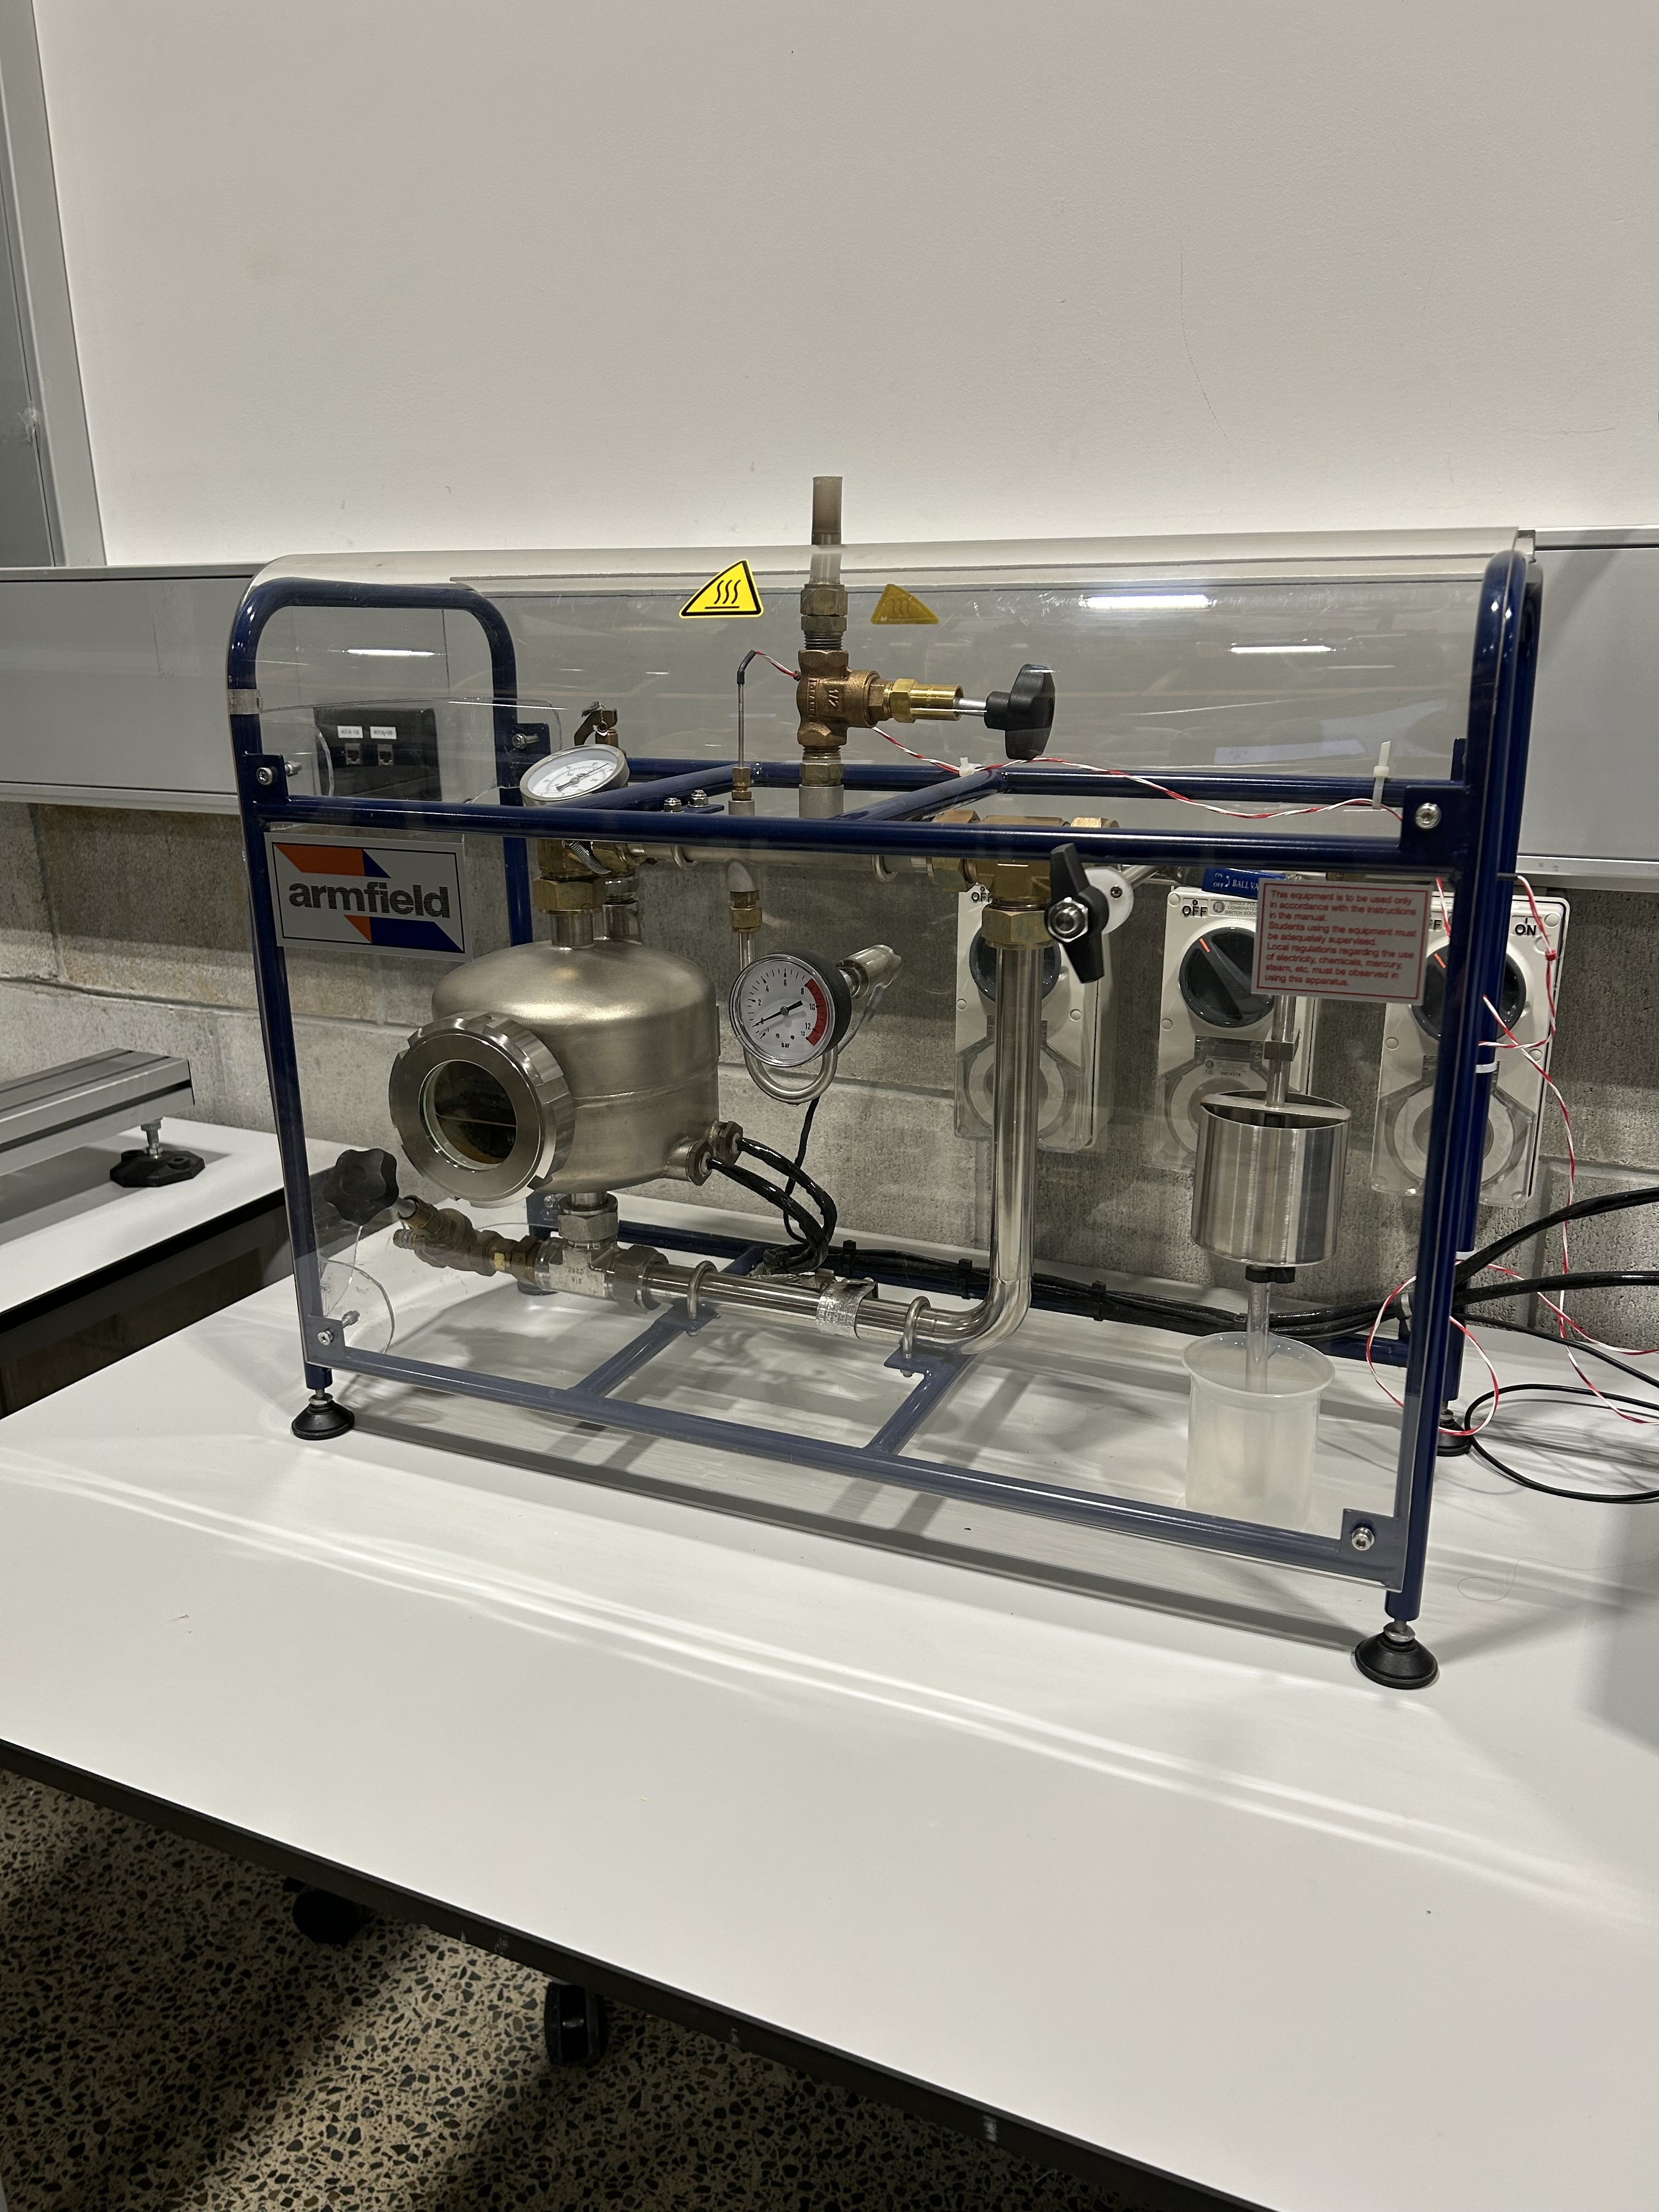
\includegraphics[width=0.90\textwidth,height=0.40\textheight,keepaspectratio]{Figure 1 - TH3 apparatus.jpeg}
  \caption{Armfield TH3 boiler and pipe loop used in the 2026 experiment. The
  photograph shows the boiler, pressure gauge, viewing port, valves and sensor
  wiring of the apparatus used.}
  \label{fig:apparatus}
\end{figure}

\section{Method}
\sectionrule
\begin{enumerate}
  \item With the drain and calorimeter isolating valves closed and console power
        off, the boiler was filled with de-ionised water to halfway up the sight glass.
  \item The water was heated to vigorous boiling with the filling point open.
        Steam was vented until the temperature indication stabilised, allowing air
        to be expelled from the loop.
  \item The filling valve was closed. The apparatus was then treated as a sealed,
        approximately constant-volume system containing a saturated water--steam
        mixture. Heater input was raised for approximately two minutes and reduced.
  \item Gauge pressure and PT100 resistance were recorded after the indication
        stabilised at nine stages from \SI{50}{\kilo\pascal} to
        \SI{450}{\kilo\pascal} gauge pressure.
  \item Gauge readings were converted to absolute pressure. Each recorded
        resistance was converted to temperature using the session-supplied
        two-point relationship documented on the laboratory whiteboard.
  \item Experimental points and direct Table A--5 values were plotted on the same
        axes and fitted separately. Theoretical temperatures were then interpolated
        at the nine experimental pressures for the point-by-point error calculation.
  \item After the final reading, the heaters were switched off and the isolating
        valve was opened before cooling to prevent a damaging partial vacuum.
\end{enumerate}

\section{Results}
\sectionrule
\subsection{Worked calculation}
For the first reading, $P_1=\SI{50.00}{\kilo\pascal}$ and
$R=\SI{142.3}{\ohm}$:
\begin{align}
 P_{\mathrm{abs}}&=50.00+101.65=\SI{151.65}{\kilo\pascal},\\
 T_{\mathrm{exp}}&=15+\frac{142.3-109.0}{0.34941}
 =110.303\,{}^\circ\mathrm{C},\\
 T_{\mathrm{th}}&=111.35+\frac{151.65-150}{175-150}(116.04-111.35)
 =111.660\,{}^\circ\mathrm{C},\\
 \mathrm{Error}&=\frac{110.303-111.660}{111.660}\times100=-1.215\%.
\end{align}

\subsection{Processed results}
\begin{table}[H]
  \centering
  \caption{Original measurements, session-derived temperatures, theoretical temperatures and errors.}
  \label{tab:results}
  \small
  \begin{tabular}{rrrrrr}
    \toprule
    $P_1$ & $P_{\mathrm{abs}}$ & $R$ & $T_{\mathrm{exp}}$ & $T_{\mathrm{th}}$ & Error \\
    (kPa) & (kPa) & ($\Omega$) & ($^\circ$C) & ($^\circ$C) & (\%) \\
    \midrule
     50 & 151.65 & 142.3 & 110.30 & 111.66 & $-1.21$ \\
    100 & 201.65 & 144.8 & 117.46 & 120.46 & $-2.49$ \\
    150 & 251.65 & 146.9 & 123.47 & 127.62 & $-3.25$ \\
    200 & 301.65 & 148.7 & 128.62 & 133.70 & $-3.80$ \\
    250 & 351.65 & 150.1 & 132.63 & 139.02 & $-4.60$ \\
    300 & 401.65 & 151.1 & 135.49 & 143.75 & $-5.75$ \\
    350 & 451.65 & 152.6 & 139.78 & 148.03 & $-5.57$ \\
    400 & 501.65 & 153.8 & 143.22 & 151.95 & $-5.75$ \\
    450 & 551.65 & 154.6 & 145.51 & 155.57 & $-6.47$ \\
    \bottomrule
  \end{tabular}
\end{table}

\subsection{Saturation curves and fitted equations}
Figure~\ref{fig:temperature} compares the processed experimental data with the
direct pressure--temperature pairs from Table A--5. Interpolated theoretical
points were not used to build either trendline.

\begin{figure}[H]
  \centering
  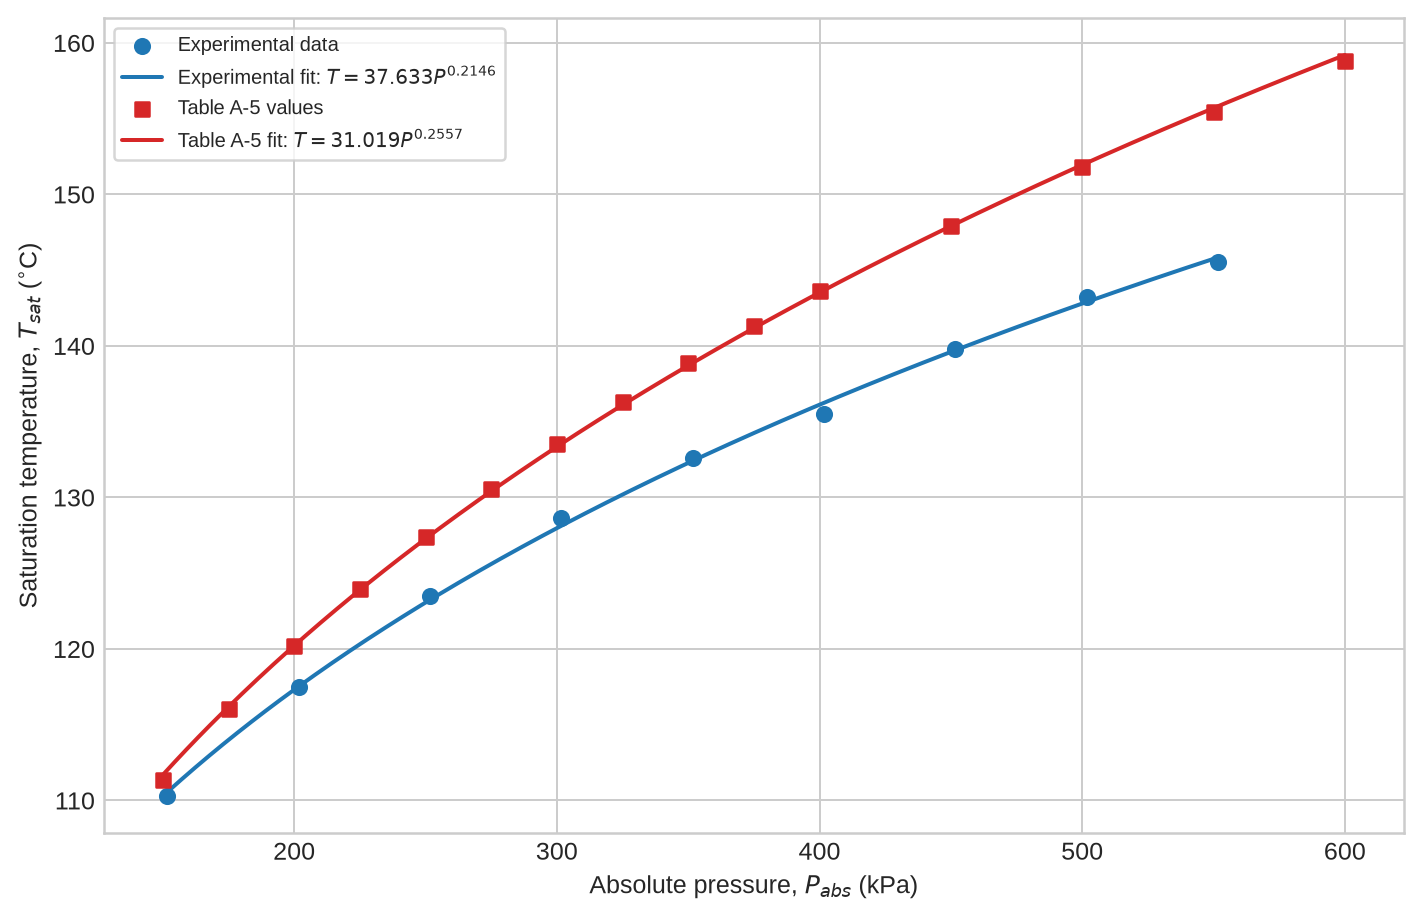
\includegraphics[width=0.78\textwidth]{Figure 2 v4 - Experimental and Table A5 values.png}
  \caption{Experimental temperatures and direct Table A--5 saturation values
  plotted against absolute pressure with separate power-law fits.}
  \label{fig:temperature}
\end{figure}

\begin{table}[H]
  \centering
  \caption{Power-law fit parameters for $T=AP^n$.}
  \label{tab:fits}
  \begin{tabular}{lrrr}
    \toprule
    Dataset & $A$ & $n$ & $R^2$ \\
    \midrule
    Experimental measurements & 37.633 & 0.2146 & 0.99895 \\
    Direct Table A--5 values & 31.019 & 0.2557 & 0.99983 \\
    \bottomrule
  \end{tabular}
\end{table}

\begin{figure}[H]
  \centering
  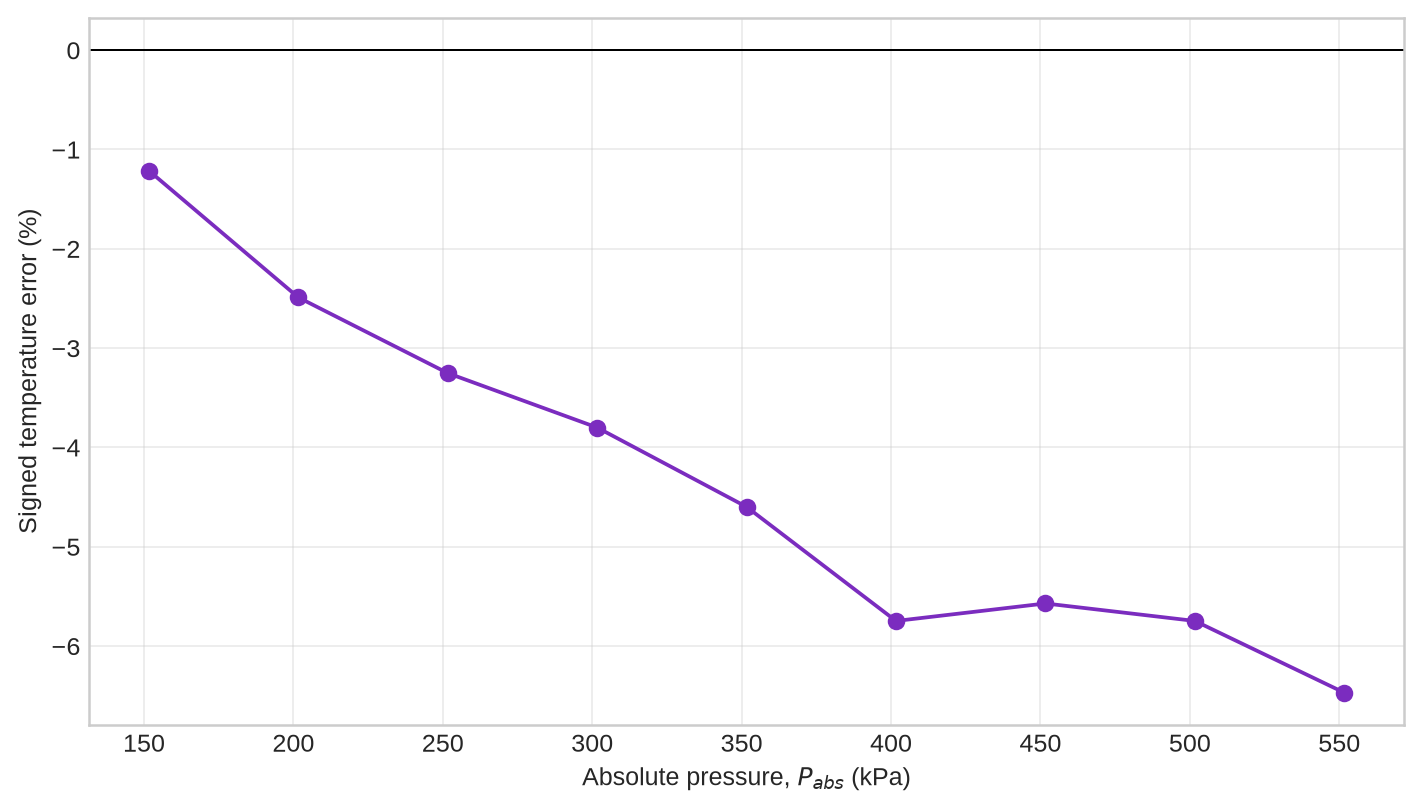
\includegraphics[width=0.56\textwidth]{Figure 3 v4 - Error versus absolute pressure.png}
  \caption{Signed experimental-temperature error relative to the point-specific
  interpolated saturation temperatures.}
  \label{fig:error}
\end{figure}

The mean signed error was $-4.32\%$. Since every value was below the reference,
the mean absolute error was also $4.32\%$. The maximum absolute error was
$6.47\%$ at \SI{551.65}{\kilo\pascal} absolute.

\section{Discussion}
\sectionrule
\subsection{Comparison and usefulness of the fitted equation}
Both curves increased smoothly with absolute pressure, confirming the expected
nonlinear relationship. However, the experimental exponent of 0.2146 was lower
than the direct-table value of 0.2557. The experimental curve therefore predicted
less temperature rise with pressure than the reference curve. Both regressions
still had $R^2>0.998$, showing that the mismatch was systematic rather than
randomly scattered.

The experimental equation is useful as a compact empirical description of
these measurements between \SI{151.65}{\kilo\pascal} and
\SI{551.65}{\kilo\pascal} absolute. It should not replace steam tables in design
work or be extrapolated outside the tested interval because it depends on the
session-supplied conversion, measurement procedure and chosen fitting method.

\subsection{Error trend}
All signed errors were negative, indicating a systematic tendency for the
derived experimental temperature to lie below the reference saturation
temperature. Error magnitude generally increased with pressure from $1.21\%$
to $6.47\%$, with a small local reduction at \SI{451.65}{\kilo\pascal}. The
trend is consistent with a pressure-dependent bias, but the experiment alone
cannot identify whether its principal cause was thermal behaviour, residual air,
instrument response or the session-supplied resistance conversion.

\subsection{Steam temperature, water temperature and assumptions}
Saturated liquid and vapour have the same temperature only at thermodynamic
equilibrium. The PT100 measured steam in the upper pipework rather than liquid
inside the boiler. The comparison therefore made the following assumptions:
\begin{itemize}
  \item air was sufficiently purged for total measured pressure to approximate
        the steam saturation pressure;
  \item pressure, boiler water, local steam and the PT100 had reached a common
        equilibrium value before each reading;
  \item atmospheric pressure remained effectively constant during the run;
  \item the whiteboard values $109.0~\Omega$ at $15\,{}^\circ\mathrm{C}$ and
        $138.7~\Omega$ at $100\,{}^\circ\mathrm{C}$ were the intended processing
        points for this session; and
  \item a straight line between those points adequately represented the recorded
        resistance range, while steam-table interpolation was adequate over the
        small pressure intervals used.
\end{itemize}
These assumptions are reasonable for processing the data, but the experiment
did not test each one independently. Consequently, the possible causes below
are interpretations consistent with the observed errors, not proven mechanisms.

Thermal lag occurs because energy must conduct through the fluid, pipework and
probe sheath before the sensor reaches the local steam temperature. Heat loss
from exposed pipework can also keep the probe region slightly cooler than the
boiler. Either effect would produce negative temperature error if a reading were
taken before complete stabilisation.

\subsection{Possible sources of error and improvements}
\begin{itemize}
  \item \textbf{Residual air:} remaining non-condensable air contributes partial
        pressure, so the measured total pressure can exceed the steam partial
        pressure associated with the local saturation temperature.
  \item \textbf{Thermal lag and heat loss:} sensor response time and temperature
        gradients can make the upper-pipe measurement lower than the equilibrium
        boiler temperature.
  \newpage
  \item \textbf{Calibration uncertainty and method sensitivity:} two defensible
        temperature-processing routes are available. The session whiteboard gives
        a two-point relation, whereas the Armfield manual specifies Data Sheet~1
        bridge correction followed by Data Sheet~2 conversion. Every recorded
        resistance ($142.3$--$154.6~\Omega$) was above the whiteboard's upper point
        of $138.7~\Omega$ at $100\,{}^\circ\mathrm{C}$. The session calculation was
        therefore an extrapolation, not an interpolation, and assumed that one
        constant slope remained valid above $100\,{}^\circ\mathrm{C}$. The available
        evidence also does not establish whether both whiteboard endpoint
        resistances were intended as indicated or bridge-corrected values; the
        manual distinguishes between these quantities. Endpoint rounding, display
        resolution and uncertainty in the stated $15\,{}^\circ\mathrm{C}$ reference
        would consequently affect every derived temperature.

        Applied to the same raw readings, the session method gives a mean signed
        error of $-4.32\%$, whereas the manual method gives $-1.03\%$. The manual
        temperatures are higher by approximately $0.75\,{}^\circ\mathrm{C}$ at the
        first point and $8.32\,{}^\circ\mathrm{C}$ at the final point. This widening
        difference demonstrates that conversion choice can create a
        pressure-dependent error trend. These two results are sensitivity cases,
        not statistical uncertainty limits; without a traceable calibration and
        repeated readings, a defensible confidence interval cannot be assigned.
        This report retains the session method because it is documented in the
        primary evidence from the actual laboratory session.
  \item \textbf{Pressure measurement:} pressure-sensor calibration, display
        resolution and atmospheric-pressure uncertainty affect absolute pressure.
  \item \textbf{Single readings:} one value at each stage cannot distinguish
        random variation, hysteresis and repeatability from systematic bias.
\end{itemize}

The experiment would be stronger if each pressure stage were repeated after
independent stabilisation. Means and standard deviations could then be reported,
and an increasing-pressure run could be compared with a decreasing-pressure run
to identify hysteresis. Longer air purging, an explicit stability criterion for
both pressure and resistance, and documented instrument resolutions would
further strengthen the uncertainty assessment.

\section{Conclusion}
\sectionrule
The experiment reproduced the expected nonlinear increase in water saturation
temperature with absolute pressure. Using the two-point resistance conversion
recorded for this laboratory session, the experimental fit was
$T=37.633P^{0.2146}$ with $R^2=0.99895$, compared with the direct steam-table fit
$T=31.019P^{0.2557}$. Experimental temperatures were below point-specific
theoretical values at all nine stages, with a mean signed error of $-4.32\%$ and
a maximum absolute error of $6.47\%$. The increasing error magnitude indicates
a systematic influence but does not prove a single cause. Thermal lag, heat loss,
residual air, pressure uncertainty and the difference between the session method
and the manufacturer's Data Sheet procedure remain plausible contributors.
Repeated measurements are recommended to quantify repeatability and help
separate experimental behaviour from conversion-method bias.

\section*{References}
{\footnotesize
\begin{enumerate}[itemsep=0pt,topsep=2pt]
  \item Y. A. \c{C}engel, M. A. Boles, and M. Kano\u{g}lu,
  \emph{Thermodynamics: An Engineering Approach}, 9th SI ed., McGraw-Hill,
  2020, Table A--5.
  \item Armfield Ltd., \emph{TH3 Saturation Pressure Apparatus Instruction Manual},
  Issue 15, Data Sheets 1--2, pp. 22--24.
  \item Auckland University of Technology, \emph{ENME 601 Saturation Temperature
  \& Pressure Lab Instructions}, 2025 update used for the 2026 laboratory.
  \item Auckland University of Technology, laboratory whiteboard and TH3 controller
  photographs, Tuesday 8--10 session, 2026.
\end{enumerate}
}

\end{document}
